% !TeX program = xelatex
\documentclass[11pt]{report}

\renewcommand{\thesection}{\arabic{section}}
\usepackage{pgfplots}
\usepackage{amsmath}
\usepackage{siunitx}
\usepackage{graphicx}
\usepackage{wrapfig}
\usepackage{subcaption}
\usepackage[siunitx, RPvoltages]{circuitikz}
\usepackage[includefoot, bottom=0.5cm, right=1.5cm, left=1.5cm, top=1.5cm]{geometry}
\usepackage{enumitem}
\usepackage{lipsum}
\usepackage{fontspec}
\usepackage{sectsty}
\usepackage{setspace}
\usepackage[]{indentfirst}
\usepackage[backend=biber, style=numeric]{biblatex}

\addbibresource{diode.bib}
\graphicspath{{images}}
\pgfplotsset{width=10cm,compat=1.9, table/search path={data}}
\defaultfontfeatures{Ligatures=TeX}
\setmainfont{Arial}
\newfontfamily{\timesNewRoman}{Times New Roman}
\newenvironment{abstractText}{\timesNewRoman\itshape}{\par}
\onehalfspacing

\begin{document}
	\title{\textbf{EEE109 Lab Report:}\\ Diodes}
	\author{Felix Lianto (2362727)\\
			[1cm]{\small Instructors: Guanying Chu, Bing Han, Jiaqi Lu}}
	\maketitle

\sectionfont{\itshape\fontsize{14pt}{15}\timesNewRoman\selectfont}
\section{Abstract}
\begin{abstractText}
	This report intends to explore the semiconductor diode in its inner workings as well as the applications that these diodes have, more specifically in rectifier circuits. This was done through a real-world lab practical with the NI Elvis III working with the 1N4001 diode, as well as simulation with LTspice, with a replicated 1N4001 diode settings. The findings of from this experiment confirms the current understanding of the semiconductor diode, in that the diode has an exponential/logarithmic relationship between its current and voltage, as well as expected output wave forms from a time-domain, transient analysis.
\end{abstractText}

\rmfamily
\sectionfont{\fontsize{14pt}{15}\rmfamily\selectfont}
\section{Introduction}
Electronics is the study of motion of charges in a gas, vacuum, or semiconductor material \autocite{neamenMicroelectronicsCircuitAnalysis2007}. As a sub-field of physics, electronics is heavily being studied upon and has practical applications in virtually every aspect of the modern day life. However, due to the vastness of the field, it has also branched into many other fields, such as the focus of this experiment, microelectronics. Defined as the study of integrated circuit technology \autocite{neamenMicroelectronicsCircuitAnalysis2007}, microelectronics has made it easier for electrical engineers to fabricate a circuit with, as the name suggests, millions of very small electronic components on semiconductor materials such as silicon \autocite{neamenMicroelectronicsCircuitAnalysis2007}. This has given rise to some of the most important technology today, used in everyday life amongst other important applications.

This report will explore one such microelectronic component known as the semiconductor diode. Mainly used as converter from AC voltage source to DC voltage, or radio signal modulation extraction, this report will investigate the diode itself and applications in rectifier circuits. A detailed research aims list can be found within the next section, while hypothesis for such aims will follow shortly after this.

\subsection{Semiconductor Diodes}
Semiconductors are materials between insulators and conductors, meaning that they don't insulate electricity nearly as well as insulators but not conductive enough to be considered conductors either. Common elemental semiconductors material used in manufacturing are silicon and germanium, however semiconductors can also be from compound materials such as Gallium Arsenide \autocite{neamenMicroelectronicsCircuitAnalysis2007}. These semiconductor materials are called intrinsic semiconductor materials, where there are no other atoms present in the crystal structure \autocite{neamenMicroelectronicsCircuitAnalysis2007}. In contrast, extrinsic semiconductor materials are the opposite, where through a method called duping, foreign atoms were introduced into the material, allowing engineers to control the concentration of free electrons in the semiconductor \autocite{neamenMicroelectronicsCircuitAnalysis2007}. \\

By doing so, these materials can be further classified into 2 types, n-type and p-type. N-type semiconductors are materials with an excess of free electrons within its region, with the 'n' in 'n-type' standing for negative, as in negative charge. Meanwhile, p-type semiconductors are materials with a deficit, thus the material is more positively charged and hence the 'p' in 'p-type'. These two materials, however, are insignificant by itself, but is much more useful when they are paired together, giving rise to the pn-junction.

The pn-junction is formed when two semiconductor materials with different charges, n-type and p-type, are placed directly next to each other. Such placement creates a depletion region, where the excess electrons meets with the deficit material, creating an electric field in the process due to a charge separation \autocite{neamenMicroelectronicsCircuitAnalysis2007}. Due to this region, a potential difference is also created by the electric field, which is more commonly known as the built-in potential barrier \autocite{neamenMicroelectronicsCircuitAnalysis2007}.

One more thing of note here is that the depletion region can grow or shrink due to the external supplied voltage, should one be connected in a circuit. If the voltage at the positive terminal is larger than the one at the negative terminal, it enters the forward bias state, where current flow would ideally, act like a short circuit. Meanwhile, if the reverse is true, then the junction would be in reverse bias, where it would ideally block current flow, similar to an open circuit. Figure \ref{pnJ} illustrates this growth-shrinkage of the pn-junction. \\
\begin{figure}[h]
	\centering
	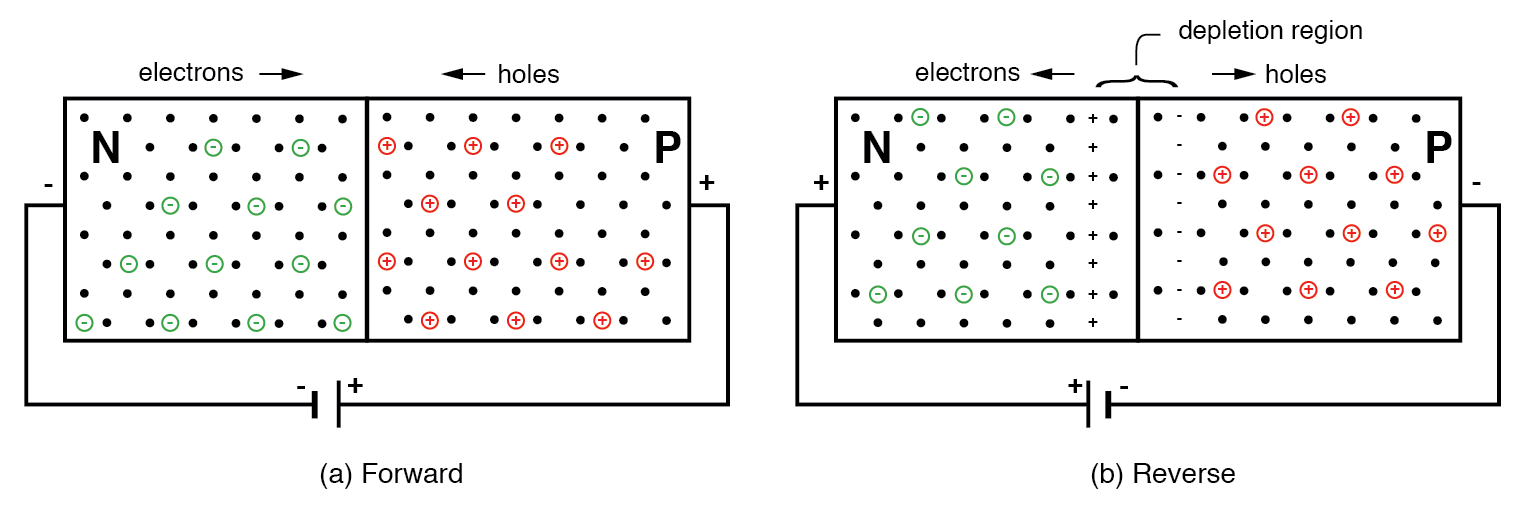
\includegraphics[scale=0.25]{pn-junction-bias.png}
	\caption{pn-junction biases. \autocite{PNJunctionSolidstate}}
	\label{pnJ}
\end{figure}

This pn-junction will serve as the regular semiconductor diode this report discusses. Other types of semiconductor diodes, such as light-emitting diodes and zener diodes are acknowledged, but will not be covered in this report. To describe the relationship between the current flowing through the diode and the diode's voltage, there are several ways to express it. One of which will be the focus for this experiment, which is the Shockley diode equation \autocite{ShockleyDiodeEquation2025},
\begin{equation}
	I_D = I_S\left(\exp\left(\frac{V_D}{nV_T}\right)-1\right)
\end{equation}
where;
\begin{align*}
	I_S &: \text{Reverse-bias saturation current,} \\
	I_D &: \text{Diode current,} \\
	n &: \text{Ideality factor,} \\
	V_T &: \text{Thermal voltage, and} \\
	V_D &: \text{Diode voltage.}
\end{align*}
To simply our discussions, however, we will be approximating the values by removing the $-1$ since its insignificant compared to the large inputs, and considering an ideal diode, where $n=1$. Hence, the final version of the ideal Shockley diode equation utilized for this report will be;
\begin{equation}
	I_D = I_S\exp\left(\frac{V_D}{V_T}\right)
\end{equation}
Thus, this experiment hypothesizes that the current-voltage relation in a diode will follow an exponential/logarithmic curve, according to the approximate ideal Shockley diode equation.

\subsection{Rectifier Circuits}
One of the most common applications of diodes in a circuit is the rectifier circuits, commonly used in converting AC voltages to DC voltages, as seen in Figure \ref{acdc}. The fundamental function of these rectifier circuits is to convert negative voltage sources into positive voltage.
\begin{figure}[h]
	\centering
	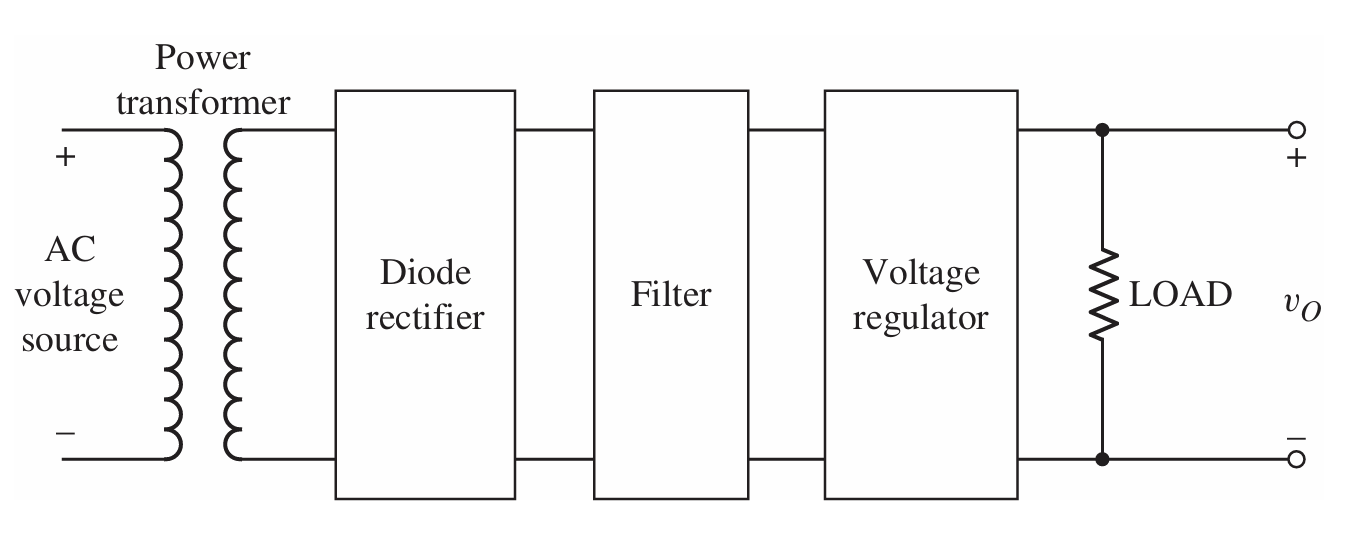
\includegraphics[scale=0.5]{acdc.png}
	\caption{The AC-DC converter circuit. \autocite{neamenMicroelectronicsCircuitAnalysis2007}}
	\label{acdc}
\end{figure}

Based on the method in which they convert these sources, two types can be inferred from this criteria, half-wave and full-wave. In a half-wave rectifier, negative voltages will ideally output as zero voltage, acting similarly to a minimum function between the input voltage and zero. On the other hand, in a full-wave rectifier, the circuit behaves more like an absolute function, where negative input voltages will result in positive output voltages with the same amplitude in an ideal case. Thus, this experiment hedges that the output waveform of these 2 circuits will be similar to the ones in Figure \ref{recCir}.
\begin{figure}[h]
	\centering
	\begin{subfigure}{0.5\textwidth}
		\centering
		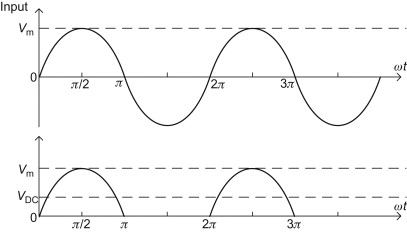
\includegraphics[scale=0.7]{halfwave.jpg}
		\caption{half-wave \autocite{gaoInterfacingESSMicrogrid2015}.}
	\end{subfigure}%
	\begin{subfigure}{0.5\textwidth}
		\centering
		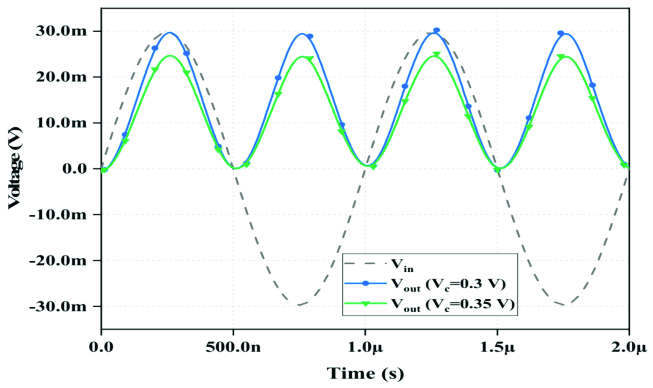
\includegraphics[scale=0.25]{fullwave.png}
		\caption{full-wave \autocite{rajElectronicallyTunableFull2021}.}
	\end{subfigure}
	\caption{Rectifier circuit signals.}
	\label{recCir}
\end{figure}

\section{Research Aims}
\textit{This experiment aims to accomplish the following objectives:}
\begin{enumerate}
	\itemsep 0em
	\item In relation to the diode,
	\begin{enumerate}
		\item understand the working principle behind the diode,
		\item observe a diode's behavior by itself, and
		\item examine the diode under a closed circuit.
	\end{enumerate}
	\item In relation to the rectifiers,
	\begin{enumerate}
		\item understand what rectifier circuits are,
		\item explore the two types of rectifier circuits, and
		\item monitor how diodes contribute to the circuits.
	\end{enumerate}
\end{enumerate}

\section{Experimental Procedure}
This experiment utilized the NI Elvis III to conduct the real-world measurements, employing the breadboard and different supplying and measuring apparatus integrated into the equipment, as well as wires and other circuit elements for the circuit construction itself. Specific details to the integrated machines and circuit elements will be mentioned in each subsection below.

Furthermore, to compare the results between real-world measurements, a nearly-identical simulation was also conducted to find the expected values to measure to. This simulation was conducted in LTspice, and was the simulated circuits were replicated to be as close to the diagrams as possible.

As mentioned previously, this section will be split according to the topics covered for this report; namely, semiconductor diodes, half-wave rectifiers, and full-wave rectifiers.

\subsection{Semiconductor Diodes}
This section of the experiment is about measuring the regular p-n junction diode and its behavior in different selected circuits. This section utilized the 1N4001 diode, a diode with a maximum repetitive peak reverse voltage of \SI{50}{\volt}, a \SI{47}{\ohm} and \SI{1}{\mega\ohm} resistor, and a \SI{1}{\kilo\ohm} potentiometer for the circuit elements.

\begin{wrapfigure}[12]{r}{0.5\textwidth}
	\centering
	\begin{circuitikz}[american, scale=1.75
		, transform shape]
		\draw (0, 0) to [vsource, l=$V$] (0, 2) 
			to [short, i=$I$] (2, 2)
			to [empty diode, l=$D$] (2, 0) -- (0, 0);
	\end{circuitikz}
	\caption{Equivalent circuit simulated in LTspice to measure the current-voltage relationship of the 1N4001 diode.}
	\label{diode}
\end{wrapfigure}

To observe the diode on its own, the IV analyzer built into the NI Elvis III equipment is deployed to measure the current-voltage relationship. The data gathered from the IV analyzer is then exported into a CSV sheet to be displayed in the upcoming results section. This data is then compared to the simulated results in LTspice, where the equivalent circuit was constructed in Figure \ref{diode} and a DC analysis sweep with identical settings was ran to produce 3 output graphs, representing the different temperatures of the diode. This experiment was ran two times on two different settings, but with the same series resistance of \SI{100}{\ohm}.

More precisely, the first DC sweep analysis is done on these settings:
\begin{align*}
	\text{Starting voltage}&: \SI{0.00}{\volt} \\
	\text{Voltage step}&: \SI{0.05}{\volt} \\
	\text{Ending voltage}&: \SI{0.70}{\volt}
\end{align*}
and the second ran on these settings:
\begin{align*}
	\text{Starting voltage}&: \SI{-10.00}{\volt} \\
	\text{Voltage step}&: \SI{0.10}{\volt} \\
	\text{Ending voltage}&: \SI{0.70}{\volt}
\end{align*}

And for measuring the diode under a closed circuit, a simple circuit featuring the potentiometer shown in Figure \ref{potDiode} was constructed on the breadboard as well as in the simulation program. Although minor adjustments to the simulation had to be committed as LTspice does not have an in-built potentiometer element, by building an equivalent circuit shown in Figure \ref{equivPotDiode} where $R$ is variable. The potentiometer was adjusted to different values, meaning different resistances, based on the voltage between the resistor and the diode, and the voltage across the diode and total current in the circuit was measured. The resulting measurements were recorded on a table and plotted onto a graph for visualization purposes.

In the simulation, the value of $R$ was decided through some elementary circuit analysis, utilizing the voltage divider formula to calculate the voltage drop $V_s$ in Figure \ref{equivPotDiode}. To explain this process in greater detail, a nodal analysis was performed on the point $S$, returning the following equation;
\begin{align*}
	\frac{1 - V_s}{1000 - R} &= \frac{V_s - 0}{R} \\
	\frac{1}{1000 - R} &= \left(\frac{1}{R} + \frac{1}{1000 - R}\right) V_s \\
	1 &= \left(\frac{1000 - R}{R} + 1\right) V_s \\
	1 &= \frac{1000}{R} V_s \\
	V_s &= \frac{R}{1000}
\end{align*}

A couple of difficulties was encountered during this portion of the experiment, for example, the potentiometer in the actual experiment had problems, in that the actual potentiometer's value did not reach the expected \SI{1}{\kilo\ohm} limit, hence the results ended abruptly near the end. Moreover, LTspice does not allow zero resistance resistor to be simulated, thus slightly different variations of the circuit in Figure \ref{equivPotDiode} was made, which only involved changing the resistor to a short circuit instead.

\begin{figure}[h]
	\centering
	\begin{subfigure}{0.5\textwidth}
		\centering
		\begin{circuitikz}[american]
			\draw (0, 0) to [vsource, l=$\SI{1}{\volt}$] (0, 4)
				to [short, -*, i=$I$] (2, 4)
				to [pR, a=$\SI{1}{\kilo\ohm}$, n=pot] (2, 1)
				to [short, -*] (2, 0) -- (0, 0);
			\draw (2, 0) to [empty diode, invert, v>=$V$] (4, 0)
				to [resistor, a=$\SI{47}{\ohm}$] (4, 2.5) -- (pot.wiper);
			\draw (2, 0) to [open, v>=$V_s$] (4, 2.5);
		\end{circuitikz}
		\caption{With potentiometer}
		\label{potDiode}
	\end{subfigure}%
	\begin{subfigure}{0.5\textwidth}
		\centering
		\begin{circuitikz}[american]
			\draw (0, 0) to [vsource, l=$\SI{1}{\volt}$] (0, 4)
				to [short, -*, i=$I$] (2, 4)
				to [resistor, l=$(\SI{1}{\kilo\ohm}) - R$, -*] (2, 2)
				to [resistor, l=$R$, v=$V_s$, -*] (2, 0) -- (0, 0);
			\draw (2, 0) to [empty diode, invert, v>=$V$] (4, 0)
				to [resistor, a=$\SI{47}{\ohm}$] (4, 2) -- (2, 2);
			\filldraw[black] (4, 2) circle (2pt) node[anchor=south]{$S$};
		\end{circuitikz}
		\caption{Equivalent circuit}
		\label{equivPotDiode}
	\end{subfigure}
	\caption{Constructed closed diode circuits}
\end{figure}

\begin{wrapfigure}[11]{l}{0.5\textwidth}
	\centering
	\begin{circuitikz}[american]
		\draw (0, 0) to [vsource, l=$\SI{10}{\volt}$] (0, 4)
			to [short, -*, i=$I$] (2, 4)
			to [pR, a=$\SI{1}{\kilo\ohm}$, n=reverse] (2, 1)
			to [short, -*] (2, 0) -- (0, 0);
		\draw (2, 0) to [empty diode, v>=$V$] (4, 0)
			to [resistor, a=$\SI{1}{\mega\ohm}$] (4, 2.5) -- (reverse.wiper);
		\draw (2, 0) to [open, v>=$V_s$] (4, 2.5);
	\end{circuitikz}
	\caption{Reversed polarity closed diode circuit}
	\label{revDiode}
\end{wrapfigure}

Finally, the experiment is reran with a bigger voltage supply of \SI{10}{\volt} and a bigger resistor of \SI{1}{\mega\ohm}, with the main focus of this experiment being the effects of swapping the diode's polarity. This circuit is illustrated in Figure \ref{revDiode}. The data collection method and subsequent visualization remains unchanged, meaning it is similar to the preceding experiment.

\subsection{Half-wave Rectifiers}
This section mainly concerns itself with an example of diode application, which are in half-wave rectifier circuits. Since rectifier circuits in general require an AC source, a function generator was used to supply said AC voltage source, while the measurement itself are read by the oscilloscope, outputting its data in the form of a CSV sheet as before. The circuit required the same diode, 1N4001, as well as a \SI{1}{\kilo\ohm} resistor to be attached in series, as illustrated in Figure \ref{halfRect}. The object of observation in this circuit was the diode voltage, which is what the data mainly comprises of.

\begin{wrapfigure}[12]{r}{0.5\textwidth}
	\centering
	\begin{circuitikz}[american, scale=1.5, transform shape]
		\draw (0, 0) -- (0, 2)
			to [empty diode, v=$V_d$] (2, 2)
			to [resistor, l=$\SI{1}{\kilo\ohm}$] (4, 2) -- (4, 0)
			to [vsourcesin, l=$V_s$] (0, 0);
	\end{circuitikz}
	\caption{Constructed half-wave rectifier circuit}
	\label{halfRect}
\end{wrapfigure}

A simulation with LTspice was also done to compare the resulting waveform. The circuit was also composed as shown in Figure \ref{halfRect}. To measure the diode voltage, a transient simulation in time-domain was done and its results from measuring the voltage across the resistor were exported into a text file to be plotted in the results and discussion section.

\subsection{Full-wave Rectifiers}
\begin{wrapfigure}{l}{0.5\textwidth}
	\centering
	\begin{circuitikz}[american]
		\draw (0, 0) to [sV=$V_s$] (0, 4) -- (4, 4)
			to [empty diode] (6, 2)
			to [resistor=$\SI{100}{\ohm}$, v=$V_r$] (2, 2)
			to [empty diode] (4, 0) -- (0, 0);
		\draw (2, 2) to [empty diode] (4, 4);
		\draw (4, 0) to [empty diode] (6, 2);
	\end{circuitikz}
	\caption{Constructed full-wave rectifier circuit}
	\label{fullRect}
\end{wrapfigure}

This segment is an extension of the previous section, which deals with a full-wave rectifier rather than half-wave. Unlike the previous section, the data gathered from this section is purely in simulation, in other words, this circuit was not tested on the breadboard. The circuit constructed in LTspice is shown in Figure \ref{fullRect}.

The data measured here is the voltage across the resistor in Figure \ref{fullRect}. Furthermore, the experiment will also compare the wave when dealing with larger resistance. Through transient time-domain simulation in LTspice, the resulting voltage values are simulated and extracted into a graph, to be discussed in the results and discussion section.

\section{Results and Discussion}
This section will present the results from the experiment, as prescribed according to the procedures in the previous section. This also includes discussion among the results, more specifically, fulfilling most of the research aims listed previously. Similar to the procedure section, the results will be comprised of two sections, the semiconductor diode and rectifier circuits.

\subsection{Semiconductor Diode}
This report promises to observe a standalone semiconductor diode through analysis by the current-voltage relationship. Figure \ref{firstSet} and \ref{secondSet} shows the experimental result and the simulation result, with 2 different settings. As expected, it does follow the exponential curve, however it is without some anomalies in the result.
\begin{figure}[h]
	\centering
	\begin{subfigure}{0.5\textwidth}
		\centering
		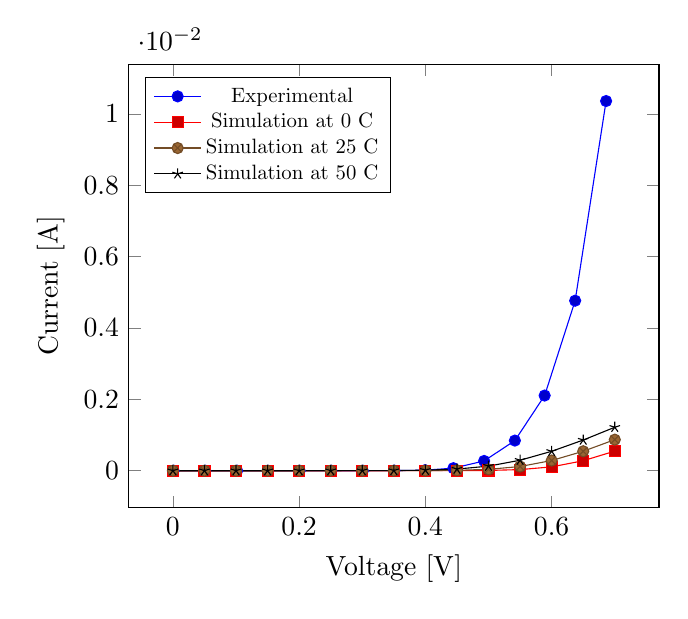
\begin{tikzpicture}
			\begin{axis}[
				xlabel={Voltage [\si{\volt}]},
				ylabel={Current [\si{\ampere}]},
				legend pos=north west,
				legend style={nodes={scale=0.75, transform shape}},
				scale=0.8,
				]
				
				% Experimental
				\addplot coordinates {
					(0.0011016973442597448,2.8072340787744457e-8)(0.05129479402550338,-2.9200020501551903e-9)(0.1017217601995741,-7.634155546221156e-8)(0.15054299672736218,-0.0000019449371102164825)(0.20078443514734648,-4.550917920670416e-7)(0.2509422554246441,-7.704342830122668e-7)(0.3007642965977152,-5.949995757531523e-7)(0.3507692524579133,0.000002357092907867564)(0.39953300151260407,0.000015225889545252836)(0.44437584359537097,0.00007090079641919045)(0.492997180500798,0.00027328840521667397)(0.5417361054193784,0.00084376089842773)(0.5888980444282247,0.0021062203215670137)(0.6372188786333721,0.004764024647920699)(0.6862504670513562,0.010358642498332547)
				};
				
				% At 0 Celcius
				\addplot coordinates {
					(0.000000000000000e+00,0.000000e+00)(5.000000000000000e-02,1.134245e-11)(1.000000000000000e-01,6.025934e-11)(1.500000000000000e-01,2.717753e-10)(2.000000000000000e-01,1.186919e-09)(2.500000000000000e-01,5.146883e-09)(3.000000000000000e-01,2.228199e-08)(3.500000000000000e-01,9.641235e-08)(4.000000000000000e-01,4.168328e-07)(4.500000000000000e-01,1.796530e-06)(4.999999999999999e-01,7.642228e-06)(5.499999999999999e-01,3.089226e-05)(6.000000000000000e-01,1.069637e-04)(6.500000000000000e-01,2.793042e-04)(7.000000000000001e-01,5.487152e-04)
				};
				
				% At 25 Celcius
				\addplot coordinates {
					(0.000000000000000e+00,0.000000e+00)(5.000000000000000e-02,1.758621e-10)(1.000000000000000e-01,8.487754e-10)(1.500000000000000e-01,3.423969e-09)(2.000000000000000e-01,1.327922e-08)(2.500000000000000e-01,5.099208e-08)(3.000000000000000e-01,1.952553e-07)(3.500000000000000e-01,7.463462e-07)(4.000000000000000e-01,2.840555e-06)(4.500000000000000e-01,1.064598e-05)(4.999999999999999e-01,3.787165e-05)(5.499999999999999e-01,1.171483e-04)(6.000000000000000e-01,2.853773e-04)(6.500000000000000e-01,5.445505e-04)(7.000000000000001e-01,8.699059e-04)
				};
				
				% At 50 Celcius
				\addplot coordinates {
					(0.000000000000000e+00,0.000000e+00)(5.000000000000000e-02,1.804056e-09)(1.000000000000000e-01,8.027314e-09)(1.500000000000000e-01,2.949428e-08)(2.000000000000000e-01,1.035319e-07)(2.500000000000000e-01,3.587334e-07)(3.000000000000000e-01,1.236642e-06)(3.500000000000000e-01,4.236279e-06)(4.000000000000000e-01,1.425738e-05)(4.500000000000000e-01,4.551989e-05)(4.999999999999999e-01,1.280066e-04)(5.499999999999999e-01,2.932329e-04)(6.000000000000000e-01,5.437806e-04)(6.500000000000000e-01,8.590126e-04)(7.000000000000001e-01,1.217906e-03)
				};
				\legend{Experimental, Simulation at 0 C, Simulation at 25 C, Simulation at 50 C}
				
			\end{axis}
		\end{tikzpicture}
		\caption{First Settings}
		\label{firstSet}
	\end{subfigure}%
	\begin{subfigure}{0.5\textwidth}
		\centering
		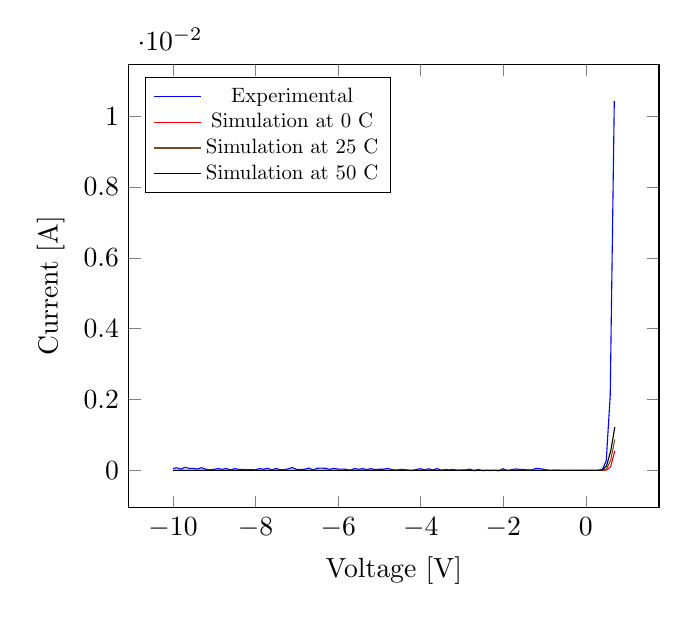
\begin{tikzpicture}
			\begin{axis}[
				xlabel={Voltage [\si{\volt}]},
				ylabel={Current [\si{\ampere}]},
				legend pos=north west,
				no markers,
				scale=0.8,
				legend style={nodes={scale=0.75, transform shape}},
				]
				
				% Experimental
				\addplot coordinates {
					(-10.003267085233164,0.000053372012772801015)(-9.908122759347219,0.0000722229336851754)(-9.80877856776502,0.000032727327410952964)(-9.709181752682298,0.00008686942862619062)(-9.60806919659641,0.000052769523513855885)(-9.50859869326395,0.000055925666809528706)(-9.4098544824955,0.000034931181197102036)(-9.310257667412769,0.00007400759808806612)(-9.209713514203074,0.00003212876978839319)(-9.106927327426188,0.000014308844689132627)(-9.00935150034768,0.00002775699569991019)(-8.908712613325276,0.0000519250425444362)(-8.808357927740966,0.000027647667772701113)(-8.708161131844491,0.000052710614651658714)(-8.608311693261237,0.00001329128196660534)(-8.508904345803911,0.00004753089913698716)(-8.407065497154008,0.000029247414583135623)(-8.306647655694569,0.000028379466683876585)(-8.208756049240396,0.000016552117164074788)(-8.106475109464572,0.000023658543524440746)(-8.007857210446389,0.000012902476714184986)(-7.90800777186314,0.0000507348444999689)(-7.808095177404756,0.00003184002041240142)(-7.706193172879722,0.00005908366950475141)(-7.606975293047777,0.000009952600583700289)(-7.508673173405253,0.00005300067057722124)(-7.4089500465722615,0.000019011559569506177)(-7.307237509672621,0.000021223981017266523)(-7.208398565091475,0.00004351757082546648)(-7.109528042572766,0.00007959942615721971)(-7.00696290135885,0.000024883286739907363)(-6.906892417212635,0.000025886179597858218)(-6.808432407882278,0.000031133601040052026)(-6.71044606761541,0.00006195323399103004)(-6.606870432399391,0.000012518385351816264)(-6.508694624507126,0.00005875285169784305)(-6.408971497674136,0.00006387041063803167)(-6.308837857652784,0.00005815136172004465)(-6.209525244008157,0.000027626289645974468)(-6.108538999672525,0.00005505223933281123)(-6.008689561089266,0.00003614788104660427)(-5.90732438150286,0.0000347818531770816)(-5.806464448917501,0.000029172447543510672)(-5.705699250144838,0.0000055981380130454285)(-5.608376046566852,0.00004913952087747475)(-5.507610847794191,0.000029411769046712167)(-5.408077188586592,0.000047322584390245835)(-5.306775164875314,0.00002254712964834482)(-5.206515213103702,0.000047619610725879725)(-5.1064447289574915,0.00002201714616039574)(-5.0081426093149615,0.00003269002218065253)(-4.907030053229072,0.00002936257866656966)(-4.808191108647927,0.00005518217969951777)(-4.707520643687958,0.000023259360521468153)(-4.606250197914243,0.0000052106146548425154)(-4.506558649018819,0.00002346581196997377)(-4.405477670870497,0.000022697973156438066)(-4.306891349789879,0.000006487849172138738)(-4.205020923202411,-0.0000053799387826991565)(-4.108487168063572,0.000027464232924243603)(-4.008795619168151,0.000045719430239437034)(-3.9077777968949583,0.000013849049153886738)(-3.8072336436852594,0.00004441372420013856)(-3.709089413730561,0.000011468444126214727)(-3.6092083972097417,0.000051549404336106444)(-3.507211658872008,0.0000031583866305417984)(-3.4082148246030304,0.000020667614810578882)(-3.3096916593975436,0.00001342325792713428)(-3.2088001488746176,0.000023845943142029037)(-3.1080981059770867,0.0000012237388378188996)(-3.0087854923324544,0.000009484790236644614)(-2.9094097228126885,0.000014549911084271728)(-2.8097813297923944,0.000034398306575660344)(-2.707942481142493,-0.000012093267776589477)(-2.6088509130608206,0.000025945236100315405)(-2.5066331291601283,-0.000009590552910645479)(-2.408583633018129,0.0000013647327900523364)(-2.3081973694962556,-0.000005918911708278074)(-2.206990079597669,0.0000013459797500203764)(-2.106003835262044,-0.00001161692641083345)(-2.007670137681951,0.00004586050205621639)(-1.9051681523431665,-0.000004698067385005001)(-1.8089817545175535,0.000016874539604987417)(-1.7112796156887784,0.0000383554208875303)(-1.6079250260357154,0.000027032233075925393)(-1.5080124315773296,0.000024485279212469457)(-1.4064577843655177,0.000009364355514545065)(-1.305787319405552,0.000009816730309724076)(-1.2081799143894747,0.00005468320296802665)(-1.1091515021829341,0.000045271294348883105)(-1.0085126151605346,0.000027768299445711797)(-0.9013301226680192,3.405590119032187e-7)(-0.8012274470705801,0.0000013351415364093454)(-0.7014004500373109,0.0000019540316137356406)(-0.6011710406923616,0.0000011636213857479927)(-0.5020796220080402,3.3815523676206107e-7)(-0.4016032778354688,-1.076822723572457e-7)(-0.30143266249709605,-1.5087388768986187e-7)(-0.2010360168667731,0.0000014081363396103996)(-0.1004577630828019,4.6085799389541937e-7)(-0.0002505648070036846,-2.0035402827219885e-7)(0.10086990037095216,-7.914552797638752e-8)(0.19954976100923638,-5.718967052825707e-7)(0.29981967289204986,-0.0000011700377610696088)(0.39866154368178996,0.00001535269953345464)(0.4926901451331199,0.00027329264686578203)(0.5889241750978144,0.002117466889884081)(0.6863654419975502,0.010332810670296963)(0.6860989091677361,0.010426831743965088)
					
				};
				
				% At 0 Celcius
				\addplot coordinates {
					(-1.000000000000000e+01,-1.336497e-11)(-9.900000000000000e+00,-1.328038e-11)(-9.800000000000001e+00,-1.319579e-11)(-9.700000000000001e+00,-1.306891e-11)(-9.600000000000001e+00,-1.298432e-11)(-9.500000000000002e+00,-1.285744e-11)(-9.400000000000002e+00,-1.281515e-11)(-9.300000000000002e+00,-1.268826e-11)(-9.200000000000003e+00,-1.260368e-11)(-9.100000000000003e+00,-1.247679e-11)(-9.000000000000004e+00,-1.234991e-11)(-8.900000000000004e+00,-1.230761e-11)(-8.800000000000004e+00,-1.218073e-11)(-8.700000000000005e+00,-1.209614e-11)(-8.600000000000005e+00,-1.196926e-11)(-8.500000000000005e+00,-1.188467e-11)(-8.400000000000006e+00,-1.175779e-11)(-8.300000000000006e+00,-1.171550e-11)(-8.200000000000006e+00,-1.158861e-11)(-8.100000000000007e+00,-1.150403e-11)(-8.000000000000007e+00,-1.137714e-11)(-7.900000000000007e+00,-1.129255e-11)(-7.800000000000008e+00,-1.118682e-11)(-7.700000000000008e+00,-1.110223e-11)(-7.600000000000009e+00,-1.099649e-11)(-7.500000000000009e+00,-1.086961e-11)(-7.400000000000009e+00,-1.078502e-11)(-7.300000000000010e+00,-1.067929e-11)(-7.200000000000010e+00,-1.057355e-11)(-7.100000000000010e+00,-1.048896e-11)(-7.000000000000011e+00,-1.038323e-11)(-6.900000000000011e+00,-1.029864e-11)(-6.800000000000011e+00,-1.019290e-11)(-6.700000000000012e+00,-1.008717e-11)(-6.600000000000012e+00,-1.000258e-11)(-6.500000000000012e+00,-9.875698e-12)(-6.400000000000013e+00,-9.769963e-12)(-6.300000000000013e+00,-9.685374e-12)(-6.200000000000014e+00,-9.579638e-12)(-6.100000000000014e+00,-9.495051e-12)(-6.000000000000014e+00,-9.389315e-12)(-5.900000000000015e+00,-9.283579e-12)(-5.800000000000015e+00,-9.198991e-12)(-5.700000000000015e+00,-9.093256e-12)(-5.600000000000016e+00,-8.987520e-12)(-5.500000000000016e+00,-8.881784e-12)(-5.400000000000016e+00,-8.776048e-12)(-5.300000000000017e+00,-8.691460e-12)(-5.200000000000017e+00,-8.585725e-12)(-5.100000000000017e+00,-8.479989e-12)(-5.000000000000018e+00,-8.395401e-12)(-4.900000000000018e+00,-8.289665e-12)(-4.800000000000018e+00,-8.183930e-12)(-4.700000000000019e+00,-8.099342e-12)(-4.600000000000019e+00,-7.993606e-12)(-4.500000000000020e+00,-7.887870e-12)(-4.400000000000020e+00,-7.782134e-12)(-4.300000000000020e+00,-7.676399e-12)(-4.200000000000021e+00,-7.591811e-12)(-4.100000000000021e+00,-7.486075e-12)(-4.000000000000021e+00,-7.390913e-12)(-3.900000000000021e+00,-7.295752e-12)(-3.800000000000021e+00,-7.190016e-12)(-3.700000000000021e+00,-7.084280e-12)(-3.600000000000021e+00,-6.989118e-12)(-3.500000000000021e+00,-6.893956e-12)(-3.400000000000021e+00,-6.788221e-12)(-3.300000000000021e+00,-6.693059e-12)(-3.200000000000021e+00,-6.587323e-12)(-3.100000000000021e+00,-6.492161e-12)(-3.000000000000020e+00,-6.386426e-12)(-2.900000000000020e+00,-6.291264e-12)(-2.800000000000020e+00,-6.196102e-12)(-2.700000000000020e+00,-6.090366e-12)(-2.600000000000020e+00,-5.984631e-12)(-2.500000000000020e+00,-5.889469e-12)(-2.400000000000020e+00,-5.794307e-12)(-2.300000000000020e+00,-5.699145e-12)(-2.200000000000020e+00,-5.582836e-12)(-2.100000000000020e+00,-5.487674e-12)(-2.000000000000020e+00,-5.392512e-12)(-1.900000000000019e+00,-5.292063e-12)(-1.800000000000019e+00,-5.191614e-12)(-1.700000000000019e+00,-5.091166e-12)(-1.600000000000019e+00,-4.990717e-12)(-1.500000000000019e+00,-4.890268e-12)(-1.400000000000019e+00,-4.795106e-12)(-1.300000000000019e+00,-4.689370e-12)(-1.200000000000019e+00,-4.594209e-12)(-1.100000000000019e+00,-4.488473e-12)(-1.000000000000019e+00,-4.393311e-12)(-9.000000000000187e-01,-4.292863e-12)(-8.000000000000187e-01,-4.192414e-12)(-7.000000000000187e-01,-4.094608e-12)(-6.000000000000187e-01,-3.994160e-12)(-5.000000000000188e-01,-3.893711e-12)(-4.000000000000188e-01,-3.793262e-12)(-3.000000000000188e-01,-3.694135e-12)(-2.000000000000188e-01,-3.584434e-12)(-1.000000000000188e-01,-3.312496e-12)(-1.879052469178077e-14,-1.887256e-24)(9.999999999998122e-02,6.025934e-11)(1.999999999999812e-01,1.186919e-09)(2.999999999999812e-01,2.228199e-08)(3.999999999999813e-01,4.168328e-07)(4.999999999999812e-01,7.642228e-06)(5.999999999999812e-01,1.069602e-04)(7.000000000000001e-01,5.487152e-04)
				};
				
				% At 25 Celcius
				\addplot coordinates {
					(-1.000000000000000e+01,-7.219621e-11)(-9.900000000000000e+00,-7.206934e-11)(-9.800000000000001e+00,-7.198474e-11)(-9.700000000000001e+00,-7.185787e-11)(-9.600000000000001e+00,-7.177327e-11)(-9.500000000000002e+00,-7.164639e-11)(-9.400000000000002e+00,-7.160410e-11)(-9.300000000000002e+00,-7.147721e-11)(-9.200000000000003e+00,-7.139263e-11)(-9.100000000000003e+00,-7.126574e-11)(-9.000000000000004e+00,-7.113886e-11)(-8.900000000000004e+00,-7.109657e-11)(-8.800000000000004e+00,-7.096969e-11)(-8.700000000000005e+00,-7.088510e-11)(-8.600000000000005e+00,-7.075821e-11)(-8.500000000000005e+00,-7.067363e-11)(-8.400000000000006e+00,-7.058903e-11)(-8.300000000000006e+00,-7.050445e-11)(-8.200000000000006e+00,-7.037756e-11)(-8.100000000000007e+00,-7.029298e-11)(-8.000000000000007e+00,-7.018724e-11)(-7.900000000000007e+00,-7.008151e-11)(-7.800000000000008e+00,-6.997577e-11)(-7.700000000000008e+00,-6.989118e-11)(-7.600000000000009e+00,-6.978545e-11)(-7.500000000000009e+00,-6.965856e-11)(-7.400000000000009e+00,-6.957398e-11)(-7.300000000000010e+00,-6.946824e-11)(-7.200000000000010e+00,-6.938365e-11)(-7.100000000000010e+00,-6.927792e-11)(-7.000000000000011e+00,-6.917218e-11)(-6.900000000000011e+00,-6.908759e-11)(-6.800000000000011e+00,-6.898185e-11)(-6.700000000000012e+00,-6.887612e-11)(-6.600000000000012e+00,-6.879153e-11)(-6.500000000000012e+00,-6.866465e-11)(-6.400000000000013e+00,-6.858007e-11)(-6.300000000000013e+00,-6.847432e-11)(-6.200000000000014e+00,-6.836859e-11)(-6.100000000000014e+00,-6.828400e-11)(-6.000000000000014e+00,-6.817827e-11)(-5.900000000000015e+00,-6.807253e-11)(-5.800000000000015e+00,-6.798794e-11)(-5.700000000000015e+00,-6.788221e-11)(-5.600000000000016e+00,-6.779762e-11)(-5.500000000000016e+00,-6.767074e-11)(-5.400000000000016e+00,-6.756500e-11)(-5.300000000000017e+00,-6.748041e-11)(-5.200000000000017e+00,-6.737468e-11)(-5.100000000000017e+00,-6.729009e-11)(-5.000000000000018e+00,-6.718436e-11)(-4.900000000000018e+00,-6.707862e-11)(-4.800000000000018e+00,-6.699403e-11)(-4.700000000000019e+00,-6.688829e-11)(-4.600000000000019e+00,-6.678256e-11)(-4.500000000000020e+00,-6.667682e-11)(-4.400000000000020e+00,-6.657109e-11)(-4.300000000000020e+00,-6.648650e-11)(-4.200000000000021e+00,-6.638076e-11)(-4.100000000000021e+00,-6.627503e-11)(-4.000000000000021e+00,-6.617987e-11)(-3.900000000000021e+00,-6.608471e-11)(-3.800000000000021e+00,-6.598954e-11)(-3.700000000000021e+00,-6.588381e-11)(-3.600000000000021e+00,-6.577807e-11)(-3.500000000000021e+00,-6.568291e-11)(-3.400000000000021e+00,-6.558774e-11)(-3.300000000000021e+00,-6.549258e-11)(-3.200000000000021e+00,-6.537627e-11)(-3.100000000000021e+00,-6.528111e-11)(-3.000000000000020e+00,-6.518595e-11)(-2.900000000000020e+00,-6.509079e-11)(-2.800000000000020e+00,-6.498505e-11)(-2.700000000000020e+00,-6.487932e-11)(-2.600000000000020e+00,-6.478416e-11)(-2.500000000000020e+00,-6.468900e-11)(-2.400000000000020e+00,-6.458326e-11)(-2.300000000000020e+00,-6.448810e-11)(-2.200000000000020e+00,-6.438236e-11)(-2.100000000000020e+00,-6.428720e-11)(-2.000000000000020e+00,-6.418675e-11)(-1.900000000000019e+00,-6.408631e-11)(-1.800000000000019e+00,-6.398585e-11)(-1.700000000000019e+00,-6.388540e-11)(-1.600000000000019e+00,-6.378496e-11)(-1.500000000000019e+00,-6.368451e-11)(-1.400000000000019e+00,-6.358934e-11)(-1.300000000000019e+00,-6.348361e-11)(-1.200000000000019e+00,-6.338845e-11)(-1.100000000000019e+00,-6.328271e-11)(-1.000000000000019e+00,-6.318491e-11)(-9.000000000000187e-01,-6.308446e-11)(-8.000000000000187e-01,-6.298401e-11)(-7.000000000000187e-01,-6.288620e-11)(-6.000000000000187e-01,-6.278840e-11)(-5.000000000000188e-01,-6.268663e-11)(-4.000000000000188e-01,-6.258486e-11)(-3.000000000000188e-01,-6.246723e-11)(-2.000000000000188e-01,-6.209649e-11)(-1.000000000000188e-01,-5.804087e-11)(-1.879052469178077e-14,-3.138404e-23)(9.999999999998122e-02,8.487754e-10)(1.999999999999812e-01,1.327922e-08)(2.999999999999812e-01,1.952553e-07)(3.999999999999813e-01,2.840555e-06)(4.999999999999812e-01,3.787165e-05)(5.999999999999812e-01,2.853772e-04)(7.000000000000001e-01,8.699059e-04)
				};
				
				% At 50 Celcius
				\addplot coordinates {
					(-1.000000000000000e+01,-7.464082e-10)(-9.900000000000000e+00,-7.462814e-10)(-9.800000000000001e+00,-7.461968e-10)(-9.700000000000001e+00,-7.460699e-10)(-9.600000000000001e+00,-7.460276e-10)(-9.500000000000002e+00,-7.459007e-10)(-9.400000000000002e+00,-7.458161e-10)(-9.300000000000002e+00,-7.456892e-10)(-9.200000000000003e+00,-7.456046e-10)(-9.100000000000003e+00,-7.455200e-10)(-9.000000000000004e+00,-7.453932e-10)(-8.900000000000004e+00,-7.453086e-10)(-8.800000000000004e+00,-7.451817e-10)(-8.700000000000005e+00,-7.450971e-10)(-8.600000000000005e+00,-7.450125e-10)(-8.500000000000005e+00,-7.449280e-10)(-8.400000000000006e+00,-7.448011e-10)(-8.300000000000006e+00,-7.447165e-10)(-8.200000000000006e+00,-7.445896e-10)(-8.100000000000007e+00,-7.445050e-10)(-8.000000000000007e+00,-7.443993e-10)(-7.900000000000007e+00,-7.443147e-10)(-7.800000000000008e+00,-7.442089e-10)(-7.700000000000008e+00,-7.441032e-10)(-7.600000000000009e+00,-7.440186e-10)(-7.500000000000009e+00,-7.438917e-10)(-7.400000000000009e+00,-7.438071e-10)(-7.300000000000010e+00,-7.437014e-10)(-7.200000000000010e+00,-7.435957e-10)(-7.100000000000010e+00,-7.435111e-10)(-7.000000000000011e+00,-7.434053e-10)(-6.900000000000011e+00,-7.432996e-10)(-6.800000000000011e+00,-7.432150e-10)(-6.700000000000012e+00,-7.431093e-10)(-6.600000000000012e+00,-7.430247e-10)(-6.500000000000012e+00,-7.428978e-10)(-6.400000000000013e+00,-7.427921e-10)(-6.300000000000013e+00,-7.427075e-10)(-6.200000000000014e+00,-7.426018e-10)(-6.100000000000014e+00,-7.425172e-10)(-6.000000000000014e+00,-7.424114e-10)(-5.900000000000015e+00,-7.423057e-10)(-5.800000000000015e+00,-7.422211e-10)(-5.700000000000015e+00,-7.421154e-10)(-5.600000000000016e+00,-7.420096e-10)(-5.500000000000016e+00,-7.419039e-10)(-5.400000000000016e+00,-7.417982e-10)(-5.300000000000017e+00,-7.417136e-10)(-5.200000000000017e+00,-7.416078e-10)(-5.100000000000017e+00,-7.415021e-10)(-5.000000000000018e+00,-7.414175e-10)(-4.900000000000018e+00,-7.413118e-10)(-4.800000000000018e+00,-7.412060e-10)(-4.700000000000019e+00,-7.411214e-10)(-4.600000000000019e+00,-7.410157e-10)(-4.500000000000020e+00,-7.409100e-10)(-4.400000000000020e+00,-7.408043e-10)(-4.300000000000020e+00,-7.406985e-10)(-4.200000000000021e+00,-7.406139e-10)(-4.100000000000021e+00,-7.405082e-10)(-4.000000000000021e+00,-7.404130e-10)(-3.900000000000021e+00,-7.403179e-10)(-3.800000000000021e+00,-7.402121e-10)(-3.700000000000021e+00,-7.401064e-10)(-3.600000000000021e+00,-7.400112e-10)(-3.500000000000021e+00,-7.399161e-10)(-3.400000000000021e+00,-7.398103e-10)(-3.300000000000021e+00,-7.397152e-10)(-3.200000000000021e+00,-7.396094e-10)(-3.100000000000021e+00,-7.395143e-10)(-3.000000000000020e+00,-7.394085e-10)(-2.900000000000020e+00,-7.393134e-10)(-2.800000000000020e+00,-7.392182e-10)(-2.700000000000020e+00,-7.391125e-10)(-2.600000000000020e+00,-7.390067e-10)(-2.500000000000020e+00,-7.389116e-10)(-2.400000000000020e+00,-7.388164e-10)(-2.300000000000020e+00,-7.387213e-10)(-2.200000000000020e+00,-7.386050e-10)(-2.100000000000020e+00,-7.385098e-10)(-2.000000000000020e+00,-7.384146e-10)(-1.900000000000019e+00,-7.383142e-10)(-1.800000000000019e+00,-7.382137e-10)(-1.700000000000019e+00,-7.381133e-10)(-1.600000000000019e+00,-7.380128e-10)(-1.500000000000019e+00,-7.379124e-10)(-1.400000000000019e+00,-7.378172e-10)(-1.300000000000019e+00,-7.377115e-10)(-1.200000000000019e+00,-7.376163e-10)(-1.100000000000019e+00,-7.375106e-10)(-1.000000000000019e+00,-7.374128e-10)(-9.000000000000187e-01,-7.373123e-10)(-8.000000000000187e-01,-7.372119e-10)(-7.000000000000187e-01,-7.371167e-10)(-6.000000000000187e-01,-7.370136e-10)(-5.000000000000188e-01,-7.369119e-10)(-4.000000000000188e-01,-7.367770e-10)(-3.000000000000188e-01,-7.362774e-10)(-2.000000000000188e-01,-7.314149e-10)(-1.000000000000188e-01,-6.746343e-10)(-1.879052469178077e-14,-3.427517e-22)(9.999999999998122e-02,8.027315e-09)(1.999999999999812e-01,1.035319e-07)(2.999999999999812e-01,1.236642e-06)(3.999999999999813e-01,1.425738e-05)(4.999999999999812e-01,1.280035e-04)(5.999999999999812e-01,5.437721e-04)(7.000000000000001e-01,1.217901e-03)
				};
				\legend{Experimental, Simulation at 0 C, Simulation at 25 C, Simulation at 50 C}
				
			\end{axis}
		\end{tikzpicture}
		\caption{Second Settings}
		\label{secondSet}
	\end{subfigure}
	\caption{Current-voltage relationship of the semiconductor diode, in 2 different settings as mentioned before}
	\label{semiIV}
\end{figure}

The simulation result follows from what was expected from the theoretical discussion, in that the current flows larger as the temperature increases. However, the experimental results from measuring the diode shows a bigger increase in current flow over voltage. This could be caused by the series resistor when measuring with the IV analyzer, which could've dampened the simulation results. Moreover, the simulation diode's settings could be inaccurate, however the report is unable to check its accuracy. \\

Moreover, this report also investigated the diode under a closed circuit, as shown in Figure \ref{potDiode}. The indicated values from measuring the diode voltage and total current in the circuit are shown in Figure \ref{sourceTotalDiode}. From the figure, it can be seen that both the experimental and simulation results grow similarly to each other. This could be because of the exponential diode equation, leading to the total current growing exponentially.

More specifically, by doing nodal analysis on the point S in Figure \ref{equivPotDiode}, we have the following equations, assuming an ideal diode;
\begin{align*}
	R &= 1000 V_s \\
	I &= V_s \left(\frac{1}{R} + \frac{1}{47}\right) \\
	V_D &= V_T \ln\left(\frac{I_D}{I_s}\right)
\end{align*}
Note that this is not plotted in the figure, as the value of $V_T$ was not measured during the experiment and $I_s$ is not known as it is very rarely used in electronic circuit design.

\begin{figure}[h]
	\centering
	\begin{subfigure}{0.5\textwidth}
		\centering
		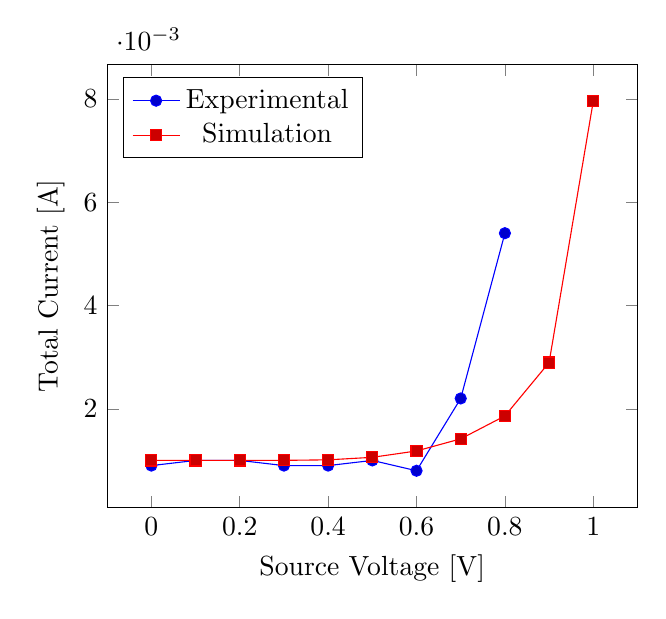
\begin{tikzpicture}
			\begin{axis}[
					xlabel={Source Voltage [$\si{\volt}$]},
					ylabel={Total Current [$\si{\ampere}$]},
					legend pos=north west,
					scale=0.8,
				]
				
				% Experimental
				\addplot coordinates {
					(0.0,0.0009)(0.1,0.001)(0.2,0.001)(0.3,0.0009)(0.4,0.0009)(0.5,0.001)(0.6,0.0008)(0.7,0.0022)(0.8,0.0054)
				};
				
				% Simulation
				\addplot coordinates {
					(0.0, 1.000000e-03)(0.1, 1.000009e-03)(0.2, 1.000136e-03)(0.3, 1.001425e-03)(0.4, 1.011640e-03)(0.5, 1.060016e-03)(0.6, 1.183339e-03)(0.7, 1.417676e-03)(0.8, 1.861873e-03)(0.9, 2.895712e-03)(1.0, 7.959051e-03)
				};
				
				\legend{Experimental, Simulation}
			\end{axis}
		\end{tikzpicture}
		\caption{Total current}
		\label{totalCurrent}
	\end{subfigure}%
	\begin{subfigure}{0.5\textwidth}
		\centering
		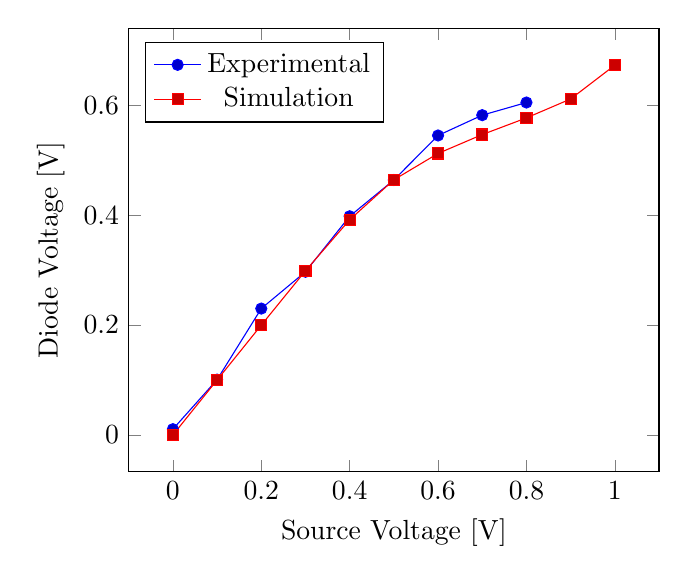
\begin{tikzpicture}
			\begin{axis}[
					xlabel={Source Voltage [$\si{\volt}$]},
					ylabel={Diode Voltage [$\si{\volt}$]},
					legend pos=north west,
					scale=0.8,
				]
				
				% Experimental
				\addplot coordinates {
					(0.0,0.0105)(0.1,0.10069)(0.2,0.23)(0.3,0.297)(0.4,0.398)(0.5,0.464)(0.6,0.545)(0.7,0.582)(0.8,0.605)
				};
				
				% Simulation
				\addplot coordinates {
					(0.0, 9.999871e-13)(0.1, 9.998836e-02)(0.2, 1.998594e-01)(0.3, 2.987788e-01)(0.4, 3.916486e-01)(0.5, 4.643504e-01)(0.6, 5.123029e-01)(0.7, 5.466533e-01)(0.8, 5.769903e-01)(0.9, 6.114305e-01)(1.0, 6.729234e-01)
				};
				
				\legend{Experimental, Simulation}
			\end{axis}
		\end{tikzpicture}
		\caption{Diode voltage}
		\label{diodeVoltage}
	\end{subfigure}
	\caption{Diode voltage and total current in relation to the source voltage}
	\label{sourceTotalDiode}
\end{figure}

Furthermore, when the diode is reversed, the following graphs in Figure \ref{revSourceTotalDiode} is produced. As expected, the reverse bias region is entered and thus the linear plots appeared in both the total current and source voltage.
\begin{figure}[h]
	\centering
	\begin{subfigure}{0.5\textwidth}
		\centering
		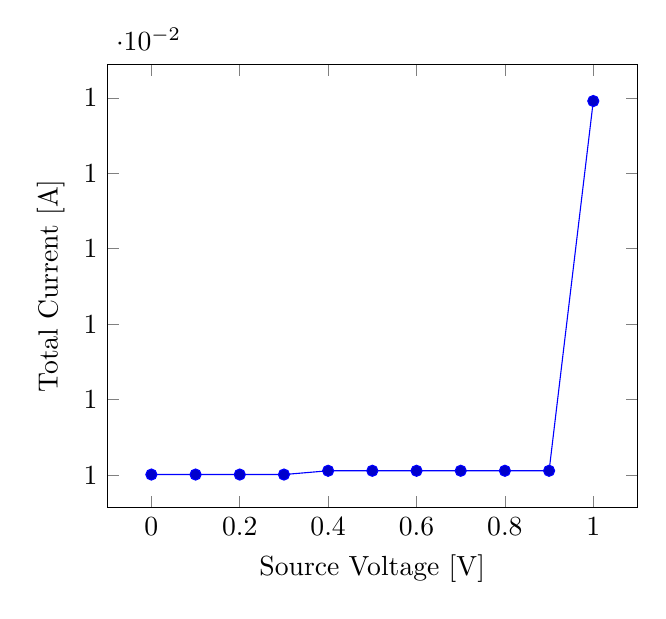
\begin{tikzpicture}
			\begin{axis}[
				xlabel={Source Voltage [$\si{\volt}$]},
				ylabel={Total Current [$\si{\ampere}$]},
				legend pos=north west,
				scale=0.8,
				]
				
				% Simulation
				\addplot coordinates {
					(0.0, 1.000000e-02)(0.1, 1.000000e-02)(0.2, 1.000000e-02)(0.3, 1.000000e-02)(0.4, 1.000001e-02)(0.5, 1.000001e-02)(0.6, 1.000001e-02)(0.7, 1.000001e-02)(0.8, 1.000001e-02)(0.9, 1.000001e-02)(1.0, 1.000099e-02)
				};
				
			\end{axis}
		\end{tikzpicture}
		\caption{Total current}
		\label{revTotalCurrent}
	\end{subfigure}%
	\begin{subfigure}{0.5\textwidth}
		\centering
		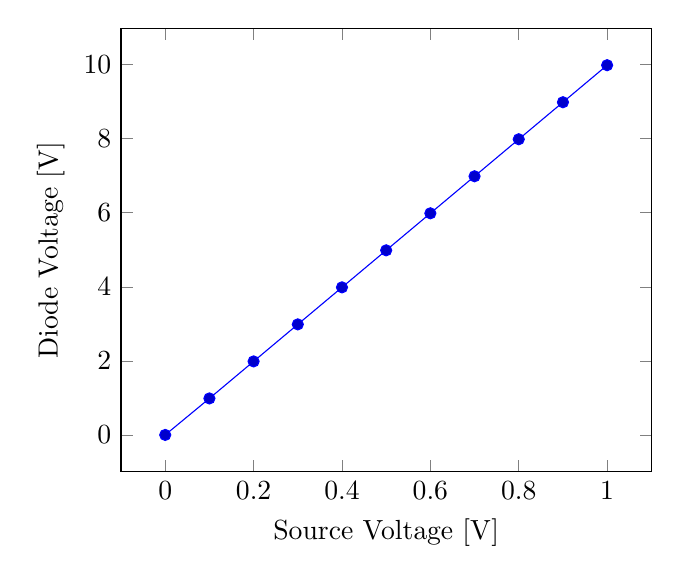
\begin{tikzpicture}
			\begin{axis}[
				xlabel={Source Voltage [$\si{\volt}$]},
				ylabel={Diode Voltage [$\si{\volt}$]},
				legend pos=north west,
				scale=0.8,
				]
				
				% Simulation
				\addplot coordinates {
					(0.0, 7.829429e-12)(0.1, 9.858878e-01)(0.2, 1.985886e+00)(0.3, 2.985884e+00)(0.4, 3.985883e+00)(0.5, 4.985881e+00)(0.6, 5.985881e+00)(0.7, 6.985880e+00)(0.8, 7.985880e+00)(0.9, 8.985880e+00)(1.0, 9.985880e+00)
				};
			\end{axis}
		\end{tikzpicture}
		\caption{Diode voltage}
		\label{revDiodeVoltage}
	\end{subfigure}
	\caption{Diode voltage and total current in relation to the source voltage}
	\label{revSourceTotalDiode}
\end{figure}

\subsection{Rectifier Circuits}
This experiment also aimed to explore diodes in rectifier circuits as one of the practical applications. Figure \ref{halfRectRes} shows the diode voltage in Figure \ref{halfRect}. From the graph, it can be concluded that both the experiment nor the simulation showed any significant difference with each other. This aligns with the hypothesis, as voltage in a diode can only have a minimum of near-zero voltage, as explained previously.
\begin{figure}[h]
	\centering
	\begin{tikzpicture}
		\begin{axis}[
				xlabel={Time [s]},
				ylabel={Voltage [V]},
				no markers,
				ymajorgrids=true,
				grid style={dashed},
				legend style={nodes={scale=0.7, transform shape}},
			]
				
			\addplot table [x=time, y=voltage, each nth point={100}] {halfwaveFull.txt};
			\addplot table [x=time, y=voltage, each nth point={100}] {halfwaveDiode.txt};
			\addplot table [x=time, y=voltage] {halfwaveSim.txt};
			
			\legend{Source, Experimental, Simulation}
		\end{axis}
	\end{tikzpicture}
	\caption{Transient time-domain simulation of the half-wave rectifier.}
	\label{halfRectRes}
\end{figure}

Furthermore, full-wave rectifiers were also explored in this experiment, although only in simulation as mentioned previously. Figure \ref{fullRectRes} shows the result from the full-wave circuit in Figure \ref{fullRect}. As expected from the theoretical discussion, the voltage across the resistor is always positive, acting similarly to an absolute function to the input wave. However, an unexpected interesting finding here is the amplitude of the voltage wave across the resistor becoming larger and larger as the resistor grows larger. This is expected, as due to the increase in resistance, current flow is much more limited the bigger the resistance is. Similar results have also been reached in other introductory microelectronic circuit analysis textbooks as well, such as Neamen \autocite{neamenMicroelectronicsCircuitAnalysis2007}. 
\begin{figure}[h]
	\centering
	\begin{tikzpicture}
		\begin{axis}[
			xlabel={Time [s]},
			ylabel={Voltage [V]},
			no markers,
			ymajorgrids=true,
			grid style={dashed},
			legend style={nodes={scale=0.7, transform shape}},
			legend pos=south west,
			]
			
			\addplot table [x=time, y=voltage] {fullwaveSource.txt};
			\addplot table [x=time, y=voltage] {fullwave100.txt};
			\addplot table [x=time, y=voltage] {fullwave100k.txt};
			\addplot table [x=time, y=voltage] {fullwave100M.txt};
			\addplot table [x=time, y=voltage] {fullwave100G.txt};
			
			\legend{Source, \SI{100}{\ohm}, \SI{100}{\kilo\ohm}, \SI{100}{\mega\ohm}, \SI{100}{\giga\ohm}}
		\end{axis}
	\end{tikzpicture}
	\caption{Transient time-domain simulation of the full-wave rectifier.}
	\label{fullRectRes}
\end{figure}

\section{Conclusion}
This experiment has explored the semiconductor diode and its applications within circuits. The report concludes that diodes are circuit elements commonly used in microelectronic circuits, working similarly to a one-way street for current flow. That is, it blocks current flow from going one way, acting more like an open circuit if it goes in the reverse direction, or more commonly known as, reverse bias. This is especially useful when manipulating with input wave forms through circuits like the rectifier circuits, which follows some voltage value while blocking others by setting its minimum to zero.

While this experiment is mostly considered successful in its research aims, there still is a lot left to be desired. Namely, with the real-world experiment portion being oftentimes hard to control due to the unpredictability of measuring something precise. In the future, it is advised that measurements are to be more precise, as the error margins when dealing with the apparatus proved to be quite large from the ideal.

Lastly, this report believes it contributes to the learning experience of the student, working with diodes in a professional manner for the first time. This experiment has enlightened the student author of this report into the field of microelectronic circuits, and motivates them to study it in greater detail and clarity.

\printbibliography

\end{document}